\documentclass[11pt,a4paper]{article}
\usepackage[utf8]{inputenc}
\usepackage[T1]{fontenc}
\usepackage{lmodern}
\usepackage[margin=2.3cm]{geometry}
\usepackage{graphicx}
\usepackage{booktabs}
\usepackage{amsmath}
\usepackage{siunitx}
\usepackage{xcolor}
\usepackage{tikz}
\usetikzlibrary{positioning,arrows.meta}
\usepackage[hidelinks]{hyperref}
\usepackage{cleveref}
\graphicspath{{../docs/img/}}

\title{Measuring Physical Plausibility of AI-Generated Training Videos\\with a Digital Twin}
\author{Sandra Elachappilly Sudhakaran\\\small M.Sc.\ Information Technology, TH OWL}
\date{November 2026}

\begin{document}
\maketitle

\begin{abstract}
Conditional video generators such as NVIDIA Cosmos-Transfer can turn a simple
simulation into realistic training and assistance videos for production. For
this use, the output must stay physically plausible: parts must not vanish,
jump, drift or change size. This report describes a pipeline that (i)~runs a
digital twin of an assembly station from a process plan, (ii)~exports depth,
segmentation and edge control videos, prompts and Cosmos-Transfer2.5 parameter
files, and (iii)~checks generated videos against the twin's ground truth with five
physics checks on top of tracking-by-detection. On 192 test videos with
known injected faults, the checks found all 60 randomly placed faults with zero
false alarms. Standard tracking metrics remained high (MOTA $\geq 0.92$ on
average) for the same faulty videos, which shows that dedicated plausibility checks are needed.
\end{abstract}

\section{Introduction}
Training and assistance content for assembly work is costly to film and goes out of date
when the product or the process changes. Digital twins already contain the product geometry and
the process sequence. Generative video models conditioned on control maps
\cite{cosmos2025,cosmostransfer2025,cosmostransfer25} can render such a twin
as realistic footage in many environments. However, video models are known to break physical
rules \cite{videophy2024,physicsiq2025}. Benchmarks for this usually rely on human ratings
or learned judges. With a digital twin, the correct motion of every part is
known, so physical plausibility can be measured directly.

This project asks: \emph{how can violations of the twin's physics in a generated video be detected
automatically, and how small a violation can be found without false alarms?}

\section{Method}

\begin{figure}[t]
\centering
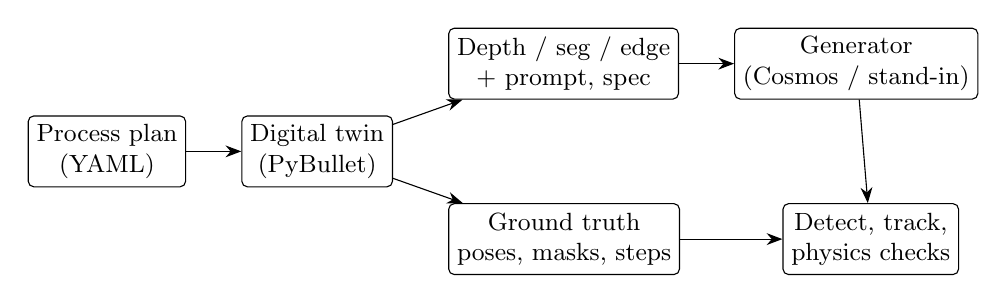
\begin{tikzpicture}[node distance=4mm and 7mm, every node/.style={font=\small},
  box/.style={draw, rounded corners=2pt, align=center, minimum height=9mm, inner sep=3pt},
  ar/.style={-{Stealth[length=2mm]}}]
\node[box] (plan) {Process plan\\(YAML)};
\node[box, right=of plan] (twin) {Digital twin\\(PyBullet)};
\node[box, above right=2mm and 7mm of twin] (ctrl) {Depth / seg / edge\\+ prompt, spec};
\node[box, below right=2mm and 7mm of twin] (gt) {Ground truth\\poses, masks, steps};
\node[box, right=of ctrl] (gen) {Generator\\(Cosmos / stand-in)};
\node[box, right=13mm of gt] (eval) {Detect, track,\\physics checks};
\draw[ar] (plan) -- (twin); \draw[ar] (twin) -- (ctrl); \draw[ar] (twin) -- (gt);
\draw[ar] (ctrl) -- (gen); \draw[ar] (gen) -- (eval); \draw[ar] (gt) -- (eval);
\end{tikzpicture}
\caption{Pipeline. The process plan is the single source of truth for the twin,
the prompts and the assistance overlay.}
\label{fig:pipeline}
\end{figure}

\paragraph{Digital twin.}
A PyBullet \cite{pybullet} scene contains a conveyor, a tray, a housing, a cover and a
gripper (\cref{fig:controls}). The process plan has six steps: the housing arrives, the cover is
picked, transferred, released \SI{2}{cm} above the housing, fastened, and the
assembly leaves. Axis moves follow minimum-jerk profiles \cite{flash1985}. After the release,
gravity and contact decide where the cover settles; a unit test checks that it comes to rest
on top of the housing (height within \SI{2}{mm}, lateral offset below \SI{5}{mm}). At \SI{24}{fps} the twin records RGB, metric depth,
a class mask, 3D poses and velocities, and the active process step for every frame.
Ground-truth 2D boxes come from the class masks after a $3\times3$ morphological opening,
which removes one- to two-pixel rendering slivers.

\paragraph{Generator inputs.}
The depth control is inverse depth normalised once per clip, so that it does not change
brightness from frame to frame. The segmentation control uses a flat colour per class and the
edge control uses Canny edges. Prompts for three visual variants are generated from the
step instructions, together with one Cosmos-Transfer2.5 parameter file per variant. A
step-annotated assistance video is rendered from the same plan.

\begin{figure}[t]
\centering
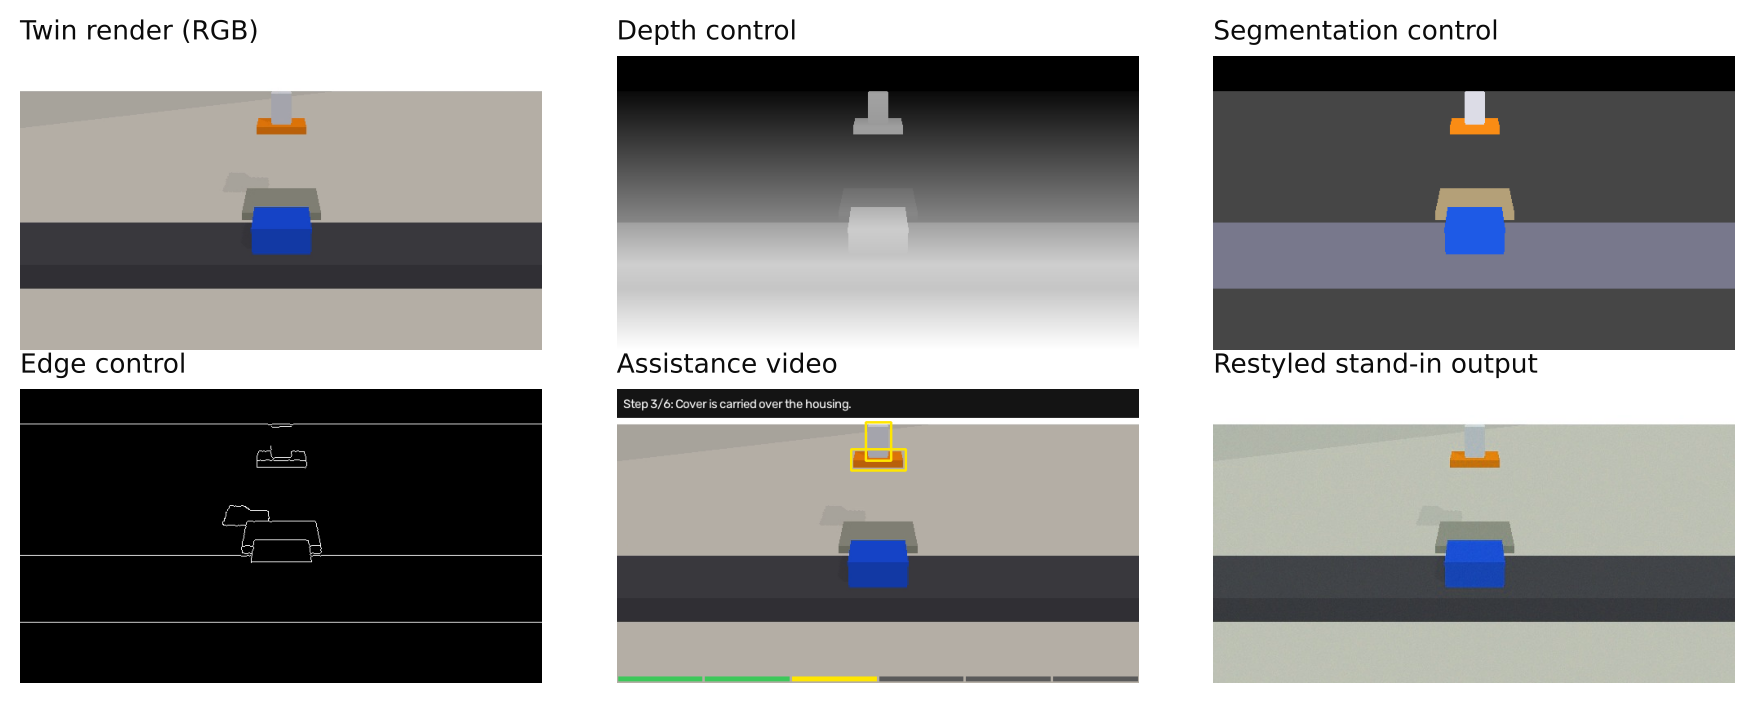
\includegraphics[width=\linewidth]{controls.png}
\caption{Twin render, the three control videos, the assistance overlay and a
restyled stand-in output (same frame).}
\label{fig:controls}
\end{figure}

\paragraph{Evaluation.}
Parts are detected by colour, since their colours are fixed by the twin and the prompt.
They are tracked with a constant-velocity Kalman filter and Hungarian
matching \cite{bewley2016sort}. The matching cost is $1-\text{IoU}$ and falls back to the
centre distance relative to the box diagonal when the boxes do not overlap. Without this
fallback the tracker lost the cover when it was lifted faster than its own height per frame.
Tracking is scored with CLEAR-MOT \cite{bernardin2008}. Let $\mathbf{c}_t$ and
$\hat{\mathbf{c}}_t$ be the detected and twin box centres. The checks are:
\begin{itemize}\itemsep0pt
\item \textbf{permanence}: the twin shows $\geq 150$ px of a part, but it is missing for $\geq 3$ frames;
\item \textbf{jump}: $\lVert \Delta\mathbf{c}_t - \Delta\hat{\mathbf{c}}_t \rVert > \SI{10}{px}$;
\item \textbf{drift}: $\lVert \mathbf{c}_t - \hat{\mathbf{c}}_t \rVert > \SI{9}{px}$ for $\geq 6$ frames;
\item \textbf{scale}: the linear box size differs from the twin by $> 25\,\%$ for $\geq 4$ frames;
\item \textbf{flicker}: the frame-to-frame change of mean background brightness differs from the twin's by $> 6$ grey levels.
\end{itemize}
Comparing \emph{changes} rather than absolute values allows the generator to restyle
the scene (lighting, colour, texture) and penalises only geometry and motion.
If the generator returns a different frame rate, the twin is sampled onto the
generator's frames. Duplicating generated frames instead produced false jumps during development.

\paragraph{Stand-in generator.}
Large video models need a datacentre GPU. To validate the checks first, the twin render is
restyled at random (channel gains $\pm10\,\%$, gamma $0.85$--$1.15$, blur, noise,
JPEG quality 70--95), which a good generator is allowed to do. One fault of known type,
object, frames and size can be injected: a part is removed (inpainted), shifted at once, shifted
gradually, scaled about its centre, or the frame brightness alternates.

\section{Results}
\Cref{tab:detection} shows 72 videos with random fault placement and severity.
Every fault was found by its check and no flag occurred outside an injected
window. The mean MOTA of the faulty videos stays between 0.92 and 1.00, and a flickering
video still scores 1.00: tracking metrics measure whether a part is found, not whether it
behaves physically.

\begin{table}[t]
\centering
\begin{tabular}{lrrrrr}
\toprule
Fault & Videos & Detected & Median latency & False alarms & Mean MOTA \\
 & & & (frames) & & \\
\midrule
clean & 12 & -- & -- & 0 & 1.000 \\
vanish & 12 & 12/12 & 0 & 0 & 0.966 \\
jump & 12 & 12/12 & 0 & 0 & 0.925 \\
drift & 12 & 12/12 & 9 & 0 & 0.964 \\
scale & 12 & 12/12 & 0 & 0 & 0.967 \\
flicker & 12 & 12/12 & 0 & 0 & 1.000 \\
\bottomrule
\end{tabular}

\caption{Fault detection on 12 videos per fault type. Latency is the
number of frames from fault start to first flag.}
\label{tab:detection}
\end{table}

\Cref{fig:sweep} sweeps the fault size (3 videos per size, 120 videos, no
false alarms). Detection starts at the thresholds: jumps of 10--12\,px, drift of
12--16\,px, size changes of 20--25\,\%, three missing frames and 2--3\,\% flicker.
Drift is detected after a median of 9 frames (\SI{0.4}{s}), because it has to rise above
the noise level first (\cref{fig:timeline}).

\begin{figure}[t]
\centering
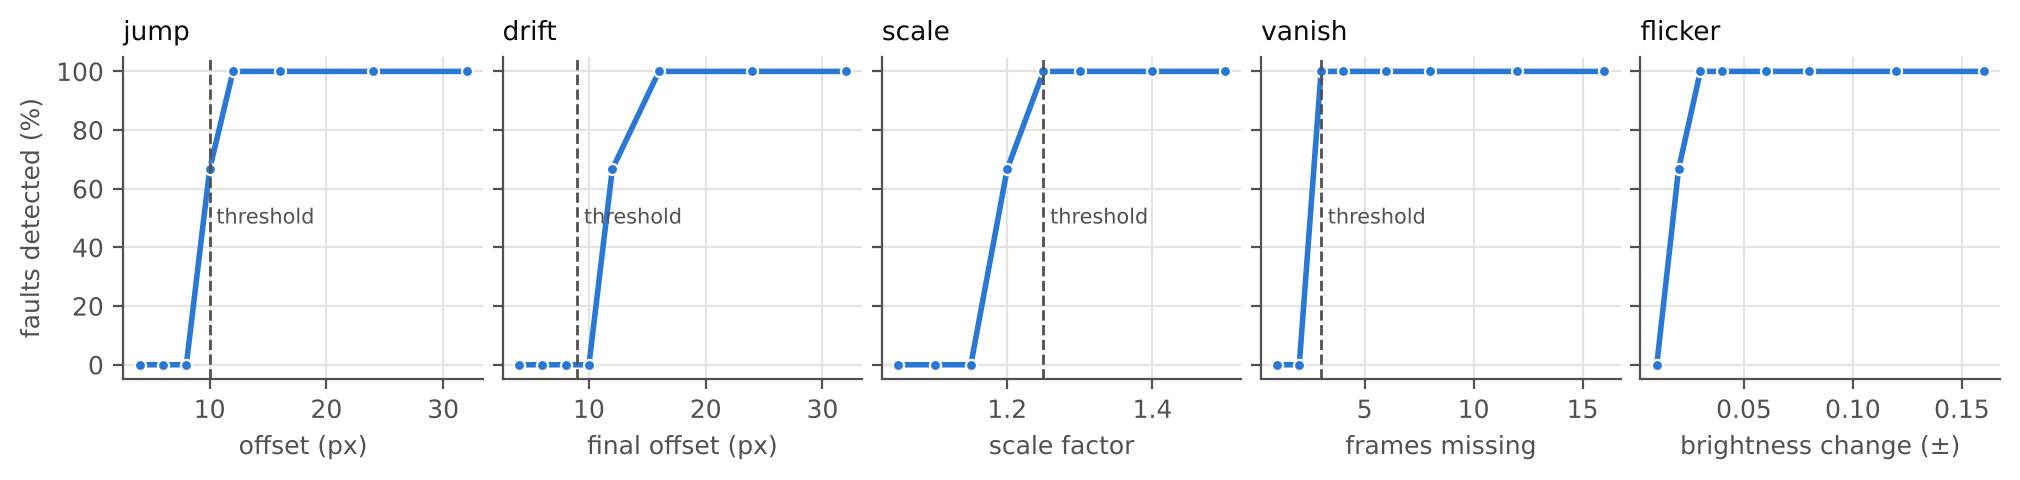
\includegraphics[width=\linewidth]{sweep.png}
\caption{Share of faults detected against fault size; dashed line: check threshold.}
\label{fig:sweep}
\end{figure}

\begin{figure}[t]
\centering
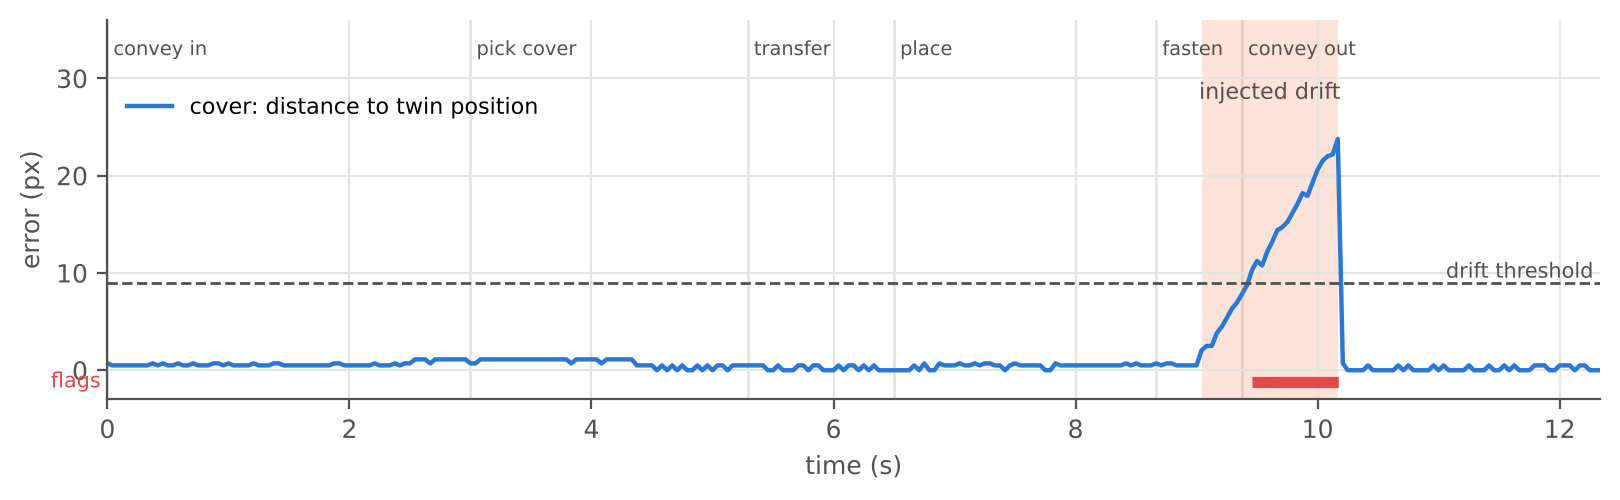
\includegraphics[width=\linewidth]{timeline.png}
\caption{Cover position error for a drift fault injected during \emph{convey out};
the red bar marks the frames flagged.}
\label{fig:timeline}
\end{figure}

\section{Limitations and Outlook}
The checks have not yet been applied to real Cosmos outputs. The next step is to run the exported
specifications on a GPU and compare control modalities and weights by the
number and type of violations they cause, and by the position error per process step.
Injected faults are simpler than real failures, which can combine deformation, motion and
invented objects. A check for objects that the twin does not contain and a 3D check using
depth estimated from the generated video are natural extensions. The colour detector should be
replaced by a learned detector (e.g.\ masks propagated from the twin's first frame) once
generators change the part colours. Pixel thresholds should be derived from the camera model.
Finally, the PyBullet scene stands in for an Omniverse/Isaac Sim twin built from CAD and
process data, which can export the same control modalities.

\bibliographystyle{plain}
\bibliography{refs}
\end{document}
